\documentclass[fleqn]{article}\usepackage[]{graphicx}\usepackage[]{color}
% maxwidth is the original width if it is less than linewidth
% otherwise use linewidth (to make sure the graphics do not exceed the margin)
\makeatletter
\def\maxwidth{ %
  \ifdim\Gin@nat@width>\linewidth
    \linewidth
  \else
    \Gin@nat@width
  \fi
}
\makeatother

\definecolor{fgcolor}{rgb}{0.345, 0.345, 0.345}
\newcommand{\hlnum}[1]{\textcolor[rgb]{0.686,0.059,0.569}{#1}}%
\newcommand{\hlstr}[1]{\textcolor[rgb]{0.192,0.494,0.8}{#1}}%
\newcommand{\hlcom}[1]{\textcolor[rgb]{0.678,0.584,0.686}{\textit{#1}}}%
\newcommand{\hlopt}[1]{\textcolor[rgb]{0,0,0}{#1}}%
\newcommand{\hlstd}[1]{\textcolor[rgb]{0.345,0.345,0.345}{#1}}%
\newcommand{\hlkwa}[1]{\textcolor[rgb]{0.161,0.373,0.58}{\textbf{#1}}}%
\newcommand{\hlkwb}[1]{\textcolor[rgb]{0.69,0.353,0.396}{#1}}%
\newcommand{\hlkwc}[1]{\textcolor[rgb]{0.333,0.667,0.333}{#1}}%
\newcommand{\hlkwd}[1]{\textcolor[rgb]{0.737,0.353,0.396}{\textbf{#1}}}%
\let\hlipl\hlkwb

\usepackage{framed}
\makeatletter
\newenvironment{kframe}{%
 \def\at@end@of@kframe{}%
 \ifinner\ifhmode%
  \def\at@end@of@kframe{\end{minipage}}%
  \begin{minipage}{\columnwidth}%
 \fi\fi%
 \def\FrameCommand##1{\hskip\@totalleftmargin \hskip-\fboxsep
 \colorbox{shadecolor}{##1}\hskip-\fboxsep
     % There is no \\@totalrightmargin, so:
     \hskip-\linewidth \hskip-\@totalleftmargin \hskip\columnwidth}%
 \MakeFramed {\advance\hsize-\width
   \@totalleftmargin\z@ \linewidth\hsize
   \@setminipage}}%
 {\par\unskip\endMakeFramed%
 \at@end@of@kframe}
\makeatother

\definecolor{shadecolor}{rgb}{.97, .97, .97}
\definecolor{messagecolor}{rgb}{0, 0, 0}
\definecolor{warningcolor}{rgb}{1, 0, 1}
\definecolor{errorcolor}{rgb}{1, 0, 0}
\newenvironment{knitrout}{}{} % an empty environment to be redefined in TeX

\usepackage{alltt}
\usepackage{amsmath}
\usepackage{amssymb}
\usepackage{geometry}
\usepackage{graphicx}
\usepackage{bm}
\usepackage{url}
\usepackage{enumerate}
\IfFileExists{upquote.sty}{\usepackage{upquote}}{}
\begin{document}

\setlength\parindent{0pt}

\Large
\textbf{Lab 5: Sampling Distributions}\\
\large
\textbf{STAT 630, Fall 2021}\\
\normalsize

\large
\textbf{Sampling Distributions using CDC Data}
\normalsize

As a demonstration of sampling distributions, we again work with the Behavioral Risk Factor Surveillance System (BRFSS) data from the CDC.  We can think of the 20000 individuals in this data set as our hypothetical ``population".  The R function \texttt{sample()} can be used to take samples of individuals from this population.

\begin{knitrout}
\definecolor{shadecolor}{rgb}{0.969, 0.969, 0.969}\color{fgcolor}\begin{kframe}
\begin{alltt}
\hlcom{# read data set into R}
\hlstd{cdc} \hlkwb{<-} \hlkwd{readRDS}\hlstd{(}\hlkwd{url}\hlstd{(}\hlstr{"https://ericwfox.github.io/data/cdc.rds"}\hlstd{))}
\end{alltt}
\end{kframe}
\end{knitrout}

Let's start by computing summary statistics and plotting the histogram and QQ plot for the weights of the 20000 individuals in the data set.

\begin{knitrout}
\definecolor{shadecolor}{rgb}{0.969, 0.969, 0.969}\color{fgcolor}\begin{kframe}
\begin{alltt}
\hlkwd{summary}\hlstd{(cdc}\hlopt{$}\hlstd{weight)}
\end{alltt}
\begin{verbatim}
##    Min. 1st Qu.  Median    Mean 3rd Qu.    Max. 
##    68.0   140.0   165.0   169.7   190.0   500.0
\end{verbatim}
\begin{alltt}
\hlkwd{par}\hlstd{(}\hlkwc{mfrow}\hlstd{=}\hlkwd{c}\hlstd{(}\hlnum{1}\hlstd{,}\hlnum{2}\hlstd{),} \hlkwc{cex}\hlstd{=}\hlnum{0.6}\hlstd{)}
\hlkwd{hist}\hlstd{(cdc}\hlopt{$}\hlstd{weight)}

\hlkwd{qqnorm}\hlstd{(cdc}\hlopt{$}\hlstd{weight)}
\hlkwd{qqline}\hlstd{(cdc}\hlopt{$}\hlstd{weight)}
\end{alltt}
\end{kframe}
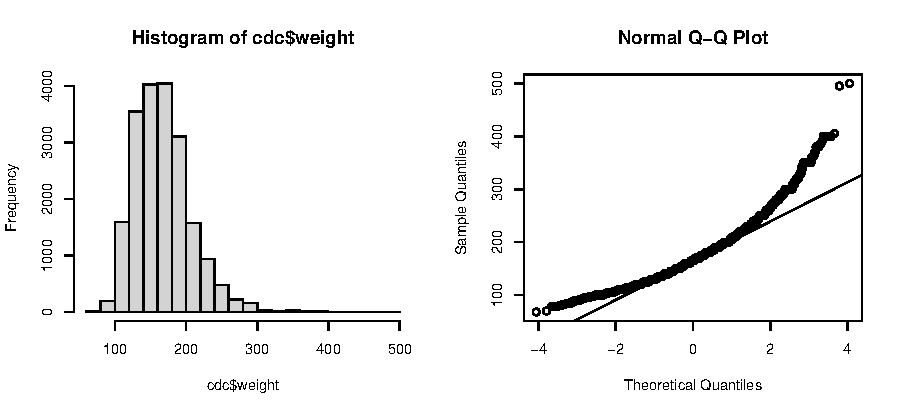
\includegraphics[width=\maxwidth]{figure/unnamed-chunk-2-1} 
\end{knitrout}

Next, use R to draw 5000 samples of size $n=30$ from this population of 20000 weights of individuals.  Compute the mean and standard deviation of the weights in each sample.  Then make a histogram and QQ plot of the 5000 sample means.  

\begin{knitrout}
\definecolor{shadecolor}{rgb}{0.969, 0.969, 0.969}\color{fgcolor}\begin{kframe}
\begin{alltt}
\hlkwd{set.seed}\hlstd{(}\hlnum{999}\hlstd{)}
\hlstd{xbars} \hlkwb{<-} \hlkwd{rep}\hlstd{(}\hlnum{0}\hlstd{,} \hlnum{5000}\hlstd{)}
\hlkwa{for}\hlstd{(i} \hlkwa{in} \hlnum{1}\hlopt{:}\hlnum{5000}\hlstd{) \{}
  \hlstd{samp} \hlkwb{<-} \hlkwd{sample}\hlstd{(cdc}\hlopt{$}\hlstd{weight,} \hlnum{30}\hlstd{)}
  \hlstd{xbars[i]} \hlkwb{<-} \hlkwd{mean}\hlstd{(samp)}
\hlstd{\}}

\hlkwd{par}\hlstd{(}\hlkwc{mfrow}\hlstd{=}\hlkwd{c}\hlstd{(}\hlnum{1}\hlstd{,}\hlnum{2}\hlstd{),} \hlkwc{cex}\hlstd{=}\hlnum{0.6}\hlstd{)}
\hlkwd{hist}\hlstd{(xbars,} \hlkwc{xlab}\hlstd{=}\hlstr{"Mean weight"}\hlstd{,} \hlkwc{main}\hlstd{=}\hlstr{"Histogram of Sample Means (n=30)"}\hlstd{)}
\hlkwd{qqnorm}\hlstd{(xbars)}
\hlkwd{qqline}\hlstd{(xbars)}
\end{alltt}
\end{kframe}
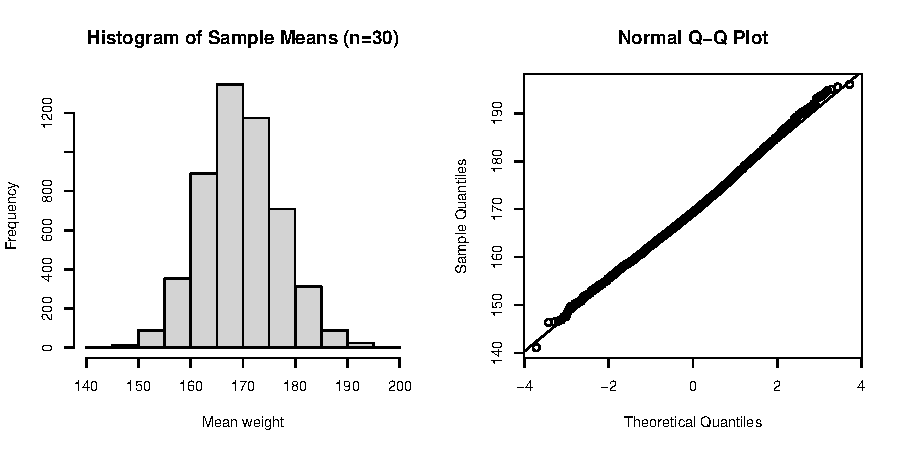
\includegraphics[width=\maxwidth]{figure/unnamed-chunk-3-1} 
\end{knitrout}

By the central limit theorem, for large $n$ (usually $n \geq 30$) the sample mean approximately follows a normal distribution centered around the mean of the population distribution $\mu$ and with standard deviation $\sigma/\sqrt{n}$, where $\sigma$ is the standard deviation of the population distribution and $n$ is the sample size.\\

Does the CLT seem to hold true for the sampling distribution generated from the CDC data set?\\
Yes -- both the QQ plot and histogram indicate that the sample means approximately follow a normal distribution.  We also have the following results for the mean and standard deviation (also called the standard error) of the sampling distribution:
\begin{knitrout}
\definecolor{shadecolor}{rgb}{0.969, 0.969, 0.969}\color{fgcolor}\begin{kframe}
\begin{alltt}
\hlkwd{mean}\hlstd{(xbars)}
\end{alltt}
\begin{verbatim}
## [1] 169.648
\end{verbatim}
\begin{alltt}
\hlkwd{mean}\hlstd{(cdc}\hlopt{$}\hlstd{weight)} \hlcom{# population mean mu}
\end{alltt}
\begin{verbatim}
## [1] 169.683
\end{verbatim}
\end{kframe}
\end{knitrout}

\newpage

\begin{knitrout}
\definecolor{shadecolor}{rgb}{0.969, 0.969, 0.969}\color{fgcolor}\begin{kframe}
\begin{alltt}
\hlkwd{sd}\hlstd{(xbars)}
\end{alltt}
\begin{verbatim}
## [1] 7.368845
\end{verbatim}
\begin{alltt}
\hlkwd{sd}\hlstd{(cdc}\hlopt{$}\hlstd{weight)} \hlopt{/} \hlkwd{sqrt}\hlstd{(}\hlnum{30}\hlstd{)} \hlcom{# sigma / sqrt(n), where sigma is population st dev}
\end{alltt}
\begin{verbatim}
## [1] 7.31775
\end{verbatim}
\end{kframe}
\end{knitrout}


\vspace{12pt}
\large
\textbf{The \texttt{for} loop}
\normalsize 

The \texttt{for} loop allows us to execute code as many times as we want without having to type out every iteration.  It is one of the most important constructs in computer science; every programming language has it's own version of the \texttt{for} loop.  While you may occasionally find a need for other types of loops (e.g., \texttt{while} loops), in my experience, I’ve found very few situations where a \texttt{for} loop wasn’t sufficient.\\

\begin{knitrout}
\definecolor{shadecolor}{rgb}{0.969, 0.969, 0.969}\color{fgcolor}\begin{kframe}
\begin{alltt}
\hlcom{# it's obviously tedious to generate a sampling distribution without using a loop:}
\hlkwd{set.seed}\hlstd{(}\hlnum{999}\hlstd{)}
\hlstd{samp1} \hlkwb{<-} \hlkwd{sample}\hlstd{(cdc}\hlopt{$}\hlstd{weight,} \hlnum{30}\hlstd{)}
\hlkwd{mean}\hlstd{(samp1)}
\end{alltt}
\begin{verbatim}
## [1] 180.8333
\end{verbatim}
\begin{alltt}
\hlstd{samp2} \hlkwb{<-} \hlkwd{sample}\hlstd{(cdc}\hlopt{$}\hlstd{weight,} \hlnum{30}\hlstd{)}
\hlkwd{mean}\hlstd{(samp2)}
\end{alltt}
\begin{verbatim}
## [1] 172
\end{verbatim}
\begin{alltt}
\hlstd{samp3} \hlkwb{<-} \hlkwd{sample}\hlstd{(cdc}\hlopt{$}\hlstd{weight,} \hlnum{30}\hlstd{)}
\hlkwd{mean}\hlstd{(samp3)}
\end{alltt}
\begin{verbatim}
## [1] 170.4
\end{verbatim}
\begin{alltt}
\hlstd{samp4} \hlkwb{<-} \hlkwd{sample}\hlstd{(cdc}\hlopt{$}\hlstd{weight,} \hlnum{30}\hlstd{)}
\hlkwd{mean}\hlstd{(samp4)}
\end{alltt}
\begin{verbatim}
## [1] 162.2667
\end{verbatim}
\begin{alltt}
\hlkwd{set.seed}\hlstd{(}\hlnum{999}\hlstd{)}
\hlstd{xbars} \hlkwb{<-} \hlkwd{rep}\hlstd{(}\hlnum{0}\hlstd{,} \hlnum{4}\hlstd{)}
\hlkwa{for}\hlstd{(i} \hlkwa{in} \hlnum{1}\hlopt{:}\hlnum{4}\hlstd{) \{}
  \hlstd{samp} \hlkwb{<-} \hlkwd{sample}\hlstd{(cdc}\hlopt{$}\hlstd{weight,} \hlnum{30}\hlstd{)}
  \hlstd{xbars[i]} \hlkwb{<-} \hlkwd{mean}\hlstd{(samp)}
\hlstd{\}}
\hlstd{xbars}
\end{alltt}
\begin{verbatim}
## [1] 180.8333 172.0000 170.4000 162.2667
\end{verbatim}
\begin{alltt}
\hlcom{# this loop prints out the variable i at each iteration}
\hlkwa{for}\hlstd{(i} \hlkwa{in} \hlnum{1}\hlopt{:}\hlnum{10}\hlstd{) \{}
  \hlkwd{print}\hlstd{(i)}
\hlstd{\}}
\end{alltt}
\begin{verbatim}
## [1] 1
## [1] 2
## [1] 3
## [1] 4
## [1] 5
## [1] 6
## [1] 7
## [1] 8
## [1] 9
## [1] 10
\end{verbatim}
\begin{alltt}
\hlcom{# some other examples demonstrating the behavior of loops in R:}
\hlstd{x} \hlkwb{<-} \hlkwd{c}\hlstd{(}\hlstr{"a"}\hlstd{,} \hlstr{"b"}\hlstd{,} \hlstr{"c"}\hlstd{,} \hlstr{"d"}\hlstd{)}
\hlkwa{for}\hlstd{(i} \hlkwa{in} \hlnum{1}\hlopt{:}\hlnum{4}\hlstd{) \{}
  \hlkwd{print}\hlstd{(x[i])}
\hlstd{\}}
\end{alltt}
\begin{verbatim}
## [1] "a"
## [1] "b"
## [1] "c"
## [1] "d"
\end{verbatim}
\begin{alltt}
\hlstd{x} \hlkwb{<-} \hlkwd{c}\hlstd{(}\hlnum{5}\hlstd{,} \hlnum{12}\hlstd{,} \hlnum{13}\hlstd{)}
\hlkwa{for}\hlstd{(n} \hlkwa{in} \hlstd{x) \{}
  \hlkwd{print}\hlstd{(n}\hlopt{^}\hlnum{2}\hlstd{)}
\hlstd{\}}
\end{alltt}
\begin{verbatim}
## [1] 25
## [1] 144
## [1] 169
\end{verbatim}
\end{kframe}
\end{knitrout}


\clearpage

\textbf{Question}: Going back to the CDC data set example, how does varying the sample size affect the sampling distribution for the mean weights?\\  

To answer this question, we use R to draw 5000 samples of size $n=5, 10, 20, 100$ from the population of 20000 weights of individuals in the CDC data set.  Again, we compute the mean of the weights in each sample; and then make histograms and QQ plots of the 5000 sample means generated for each sample size.

\begin{knitrout}
\definecolor{shadecolor}{rgb}{0.969, 0.969, 0.969}\color{fgcolor}\begin{kframe}
\begin{alltt}
\hlkwd{set.seed}\hlstd{(}\hlnum{999}\hlstd{)}
\hlstd{xbars5} \hlkwb{<-} \hlkwd{rep}\hlstd{(}\hlnum{0}\hlstd{,} \hlnum{5000}\hlstd{)}
\hlstd{xbars10} \hlkwb{<-} \hlkwd{rep}\hlstd{(}\hlnum{0}\hlstd{,} \hlnum{5000}\hlstd{)}
\hlstd{xbars20} \hlkwb{<-} \hlkwd{rep}\hlstd{(}\hlnum{0}\hlstd{,} \hlnum{5000}\hlstd{)}
\hlstd{xbars100} \hlkwb{<-} \hlkwd{rep}\hlstd{(}\hlnum{0}\hlstd{,} \hlnum{5000}\hlstd{)}
\hlkwa{for}\hlstd{(i} \hlkwa{in} \hlnum{1}\hlopt{:}\hlnum{5000}\hlstd{) \{}
  \hlstd{samp5} \hlkwb{<-} \hlkwd{sample}\hlstd{(cdc}\hlopt{$}\hlstd{weight,} \hlnum{5}\hlstd{)}
  \hlstd{xbars5[i]} \hlkwb{<-} \hlkwd{mean}\hlstd{(samp5)}

  \hlstd{samp10} \hlkwb{<-} \hlkwd{sample}\hlstd{(cdc}\hlopt{$}\hlstd{weight,} \hlnum{10}\hlstd{)}
  \hlstd{xbars10[i]} \hlkwb{<-} \hlkwd{mean}\hlstd{(samp10)}

  \hlstd{samp20} \hlkwb{<-} \hlkwd{sample}\hlstd{(cdc}\hlopt{$}\hlstd{weight,} \hlnum{20}\hlstd{)}
  \hlstd{xbars20[i]} \hlkwb{<-} \hlkwd{mean}\hlstd{(samp20)}

  \hlstd{samp100} \hlkwb{<-} \hlkwd{sample}\hlstd{(cdc}\hlopt{$}\hlstd{weight,} \hlnum{100}\hlstd{)}
  \hlstd{xbars100[i]} \hlkwb{<-} \hlkwd{mean}\hlstd{(samp100)}
\hlstd{\}}

\hlkwd{par}\hlstd{(}\hlkwc{mfrow}\hlstd{=}\hlkwd{c}\hlstd{(}\hlnum{2}\hlstd{,}\hlnum{2}\hlstd{),} \hlkwc{cex}\hlstd{=}\hlnum{0.75}\hlstd{)}
\hlkwd{hist}\hlstd{(xbars5,} \hlkwc{xlim}\hlstd{=}\hlkwd{c}\hlstd{(}\hlnum{110}\hlstd{,} \hlnum{260}\hlstd{),} \hlkwc{xaxt}\hlstd{=}\hlstr{"n"}\hlstd{,} \hlkwc{main} \hlstd{=} \hlstr{"n=5"}\hlstd{)}
\hlkwd{axis}\hlstd{(}\hlkwc{side}\hlstd{=}\hlnum{1}\hlstd{,} \hlkwc{at}\hlstd{=}\hlkwd{seq}\hlstd{(}\hlnum{100}\hlstd{,} \hlnum{250}\hlstd{,} \hlnum{25}\hlstd{),} \hlkwc{labels}\hlstd{=}\hlkwd{seq}\hlstd{(}\hlnum{100}\hlstd{,} \hlnum{250}\hlstd{,} \hlnum{25}\hlstd{))}
\hlkwd{hist}\hlstd{(xbars10,} \hlkwc{xlim}\hlstd{=}\hlkwd{c}\hlstd{(}\hlnum{110}\hlstd{,} \hlnum{260}\hlstd{),} \hlkwc{xaxt}\hlstd{=}\hlstr{"n"}\hlstd{,} \hlkwc{main} \hlstd{=} \hlstr{"n=10"}\hlstd{)}
\hlkwd{axis}\hlstd{(}\hlkwc{side}\hlstd{=}\hlnum{1}\hlstd{,} \hlkwc{at}\hlstd{=}\hlkwd{seq}\hlstd{(}\hlnum{100}\hlstd{,} \hlnum{250}\hlstd{,} \hlnum{25}\hlstd{),} \hlkwc{labels}\hlstd{=}\hlkwd{seq}\hlstd{(}\hlnum{100}\hlstd{,} \hlnum{250}\hlstd{,} \hlnum{25}\hlstd{))}
\hlkwd{hist}\hlstd{(xbars20,} \hlkwc{xlim}\hlstd{=}\hlkwd{c}\hlstd{(}\hlnum{110}\hlstd{,} \hlnum{260}\hlstd{),} \hlkwc{xaxt}\hlstd{=}\hlstr{"n"}\hlstd{,} \hlkwc{main} \hlstd{=} \hlstr{"n=20"}\hlstd{)}
\hlkwd{axis}\hlstd{(}\hlkwc{side}\hlstd{=}\hlnum{1}\hlstd{,} \hlkwc{at}\hlstd{=}\hlkwd{seq}\hlstd{(}\hlnum{100}\hlstd{,} \hlnum{250}\hlstd{,} \hlnum{25}\hlstd{),} \hlkwc{labels}\hlstd{=}\hlkwd{seq}\hlstd{(}\hlnum{100}\hlstd{,} \hlnum{250}\hlstd{,} \hlnum{25}\hlstd{))}
\hlkwd{hist}\hlstd{(xbars100,} \hlkwc{xlim}\hlstd{=}\hlkwd{c}\hlstd{(}\hlnum{110}\hlstd{,} \hlnum{260}\hlstd{),} \hlkwc{xaxt}\hlstd{=}\hlstr{"n"}\hlstd{,} \hlkwc{main} \hlstd{=} \hlstr{"n=100"}\hlstd{)}
\hlkwd{axis}\hlstd{(}\hlkwc{side}\hlstd{=}\hlnum{1}\hlstd{,} \hlkwc{at}\hlstd{=}\hlkwd{seq}\hlstd{(}\hlnum{100}\hlstd{,} \hlnum{250}\hlstd{,} \hlnum{25}\hlstd{),} \hlkwc{labels}\hlstd{=}\hlkwd{seq}\hlstd{(}\hlnum{100}\hlstd{,} \hlnum{250}\hlstd{,} \hlnum{25}\hlstd{))}
\end{alltt}
\end{kframe}
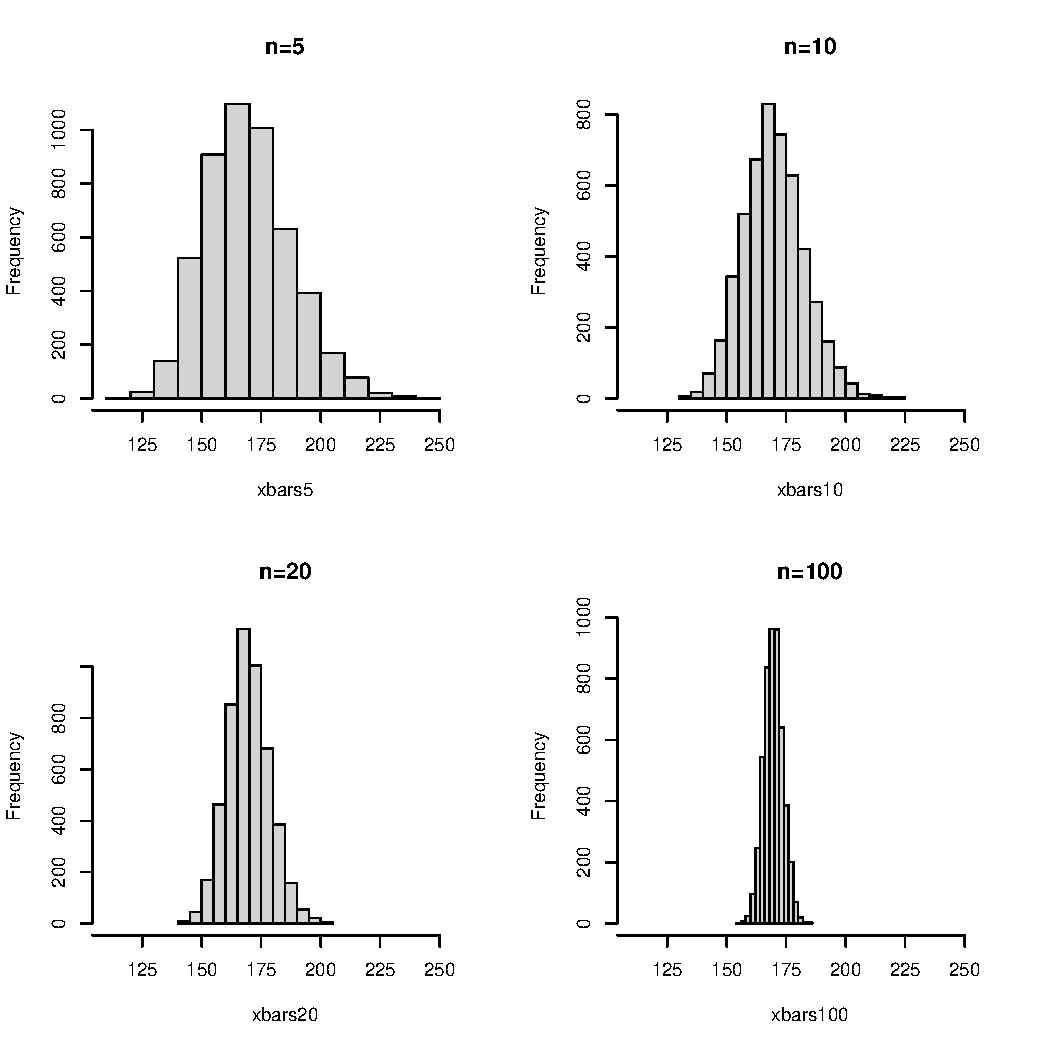
\includegraphics[width=\maxwidth]{figure/unnamed-chunk-7-1} 
\end{knitrout}
\clearpage

\begin{knitrout}
\definecolor{shadecolor}{rgb}{0.969, 0.969, 0.969}\color{fgcolor}\begin{kframe}
\begin{alltt}
\hlkwd{par}\hlstd{(}\hlkwc{mfrow}\hlstd{=}\hlkwd{c}\hlstd{(}\hlnum{2}\hlstd{,}\hlnum{2}\hlstd{),} \hlkwc{cex}\hlstd{=}\hlnum{0.75}\hlstd{)}
\hlkwd{qqnorm}\hlstd{(xbars5,} \hlkwc{main}\hlstd{=}\hlstr{"Normal Q-Q Plot (n=5)"}\hlstd{)}
\hlkwd{qqline}\hlstd{(xbars5)}
\hlkwd{qqnorm}\hlstd{(xbars10,} \hlkwc{main}\hlstd{=}\hlstr{"Normal Q-Q Plot (n=10)"}\hlstd{)}
\hlkwd{qqline}\hlstd{(xbars10)}
\hlkwd{qqnorm}\hlstd{(xbars20,} \hlkwc{main}\hlstd{=}\hlstr{"Normal Q-Q Plot (n=20)"}\hlstd{)}
\hlkwd{qqline}\hlstd{(xbars20)}
\hlkwd{qqnorm}\hlstd{(xbars100,} \hlkwc{main}\hlstd{=}\hlstr{"Normal Q-Q Plot (n=100)"}\hlstd{)}
\hlkwd{qqline}\hlstd{(xbars100)}
\end{alltt}
\end{kframe}
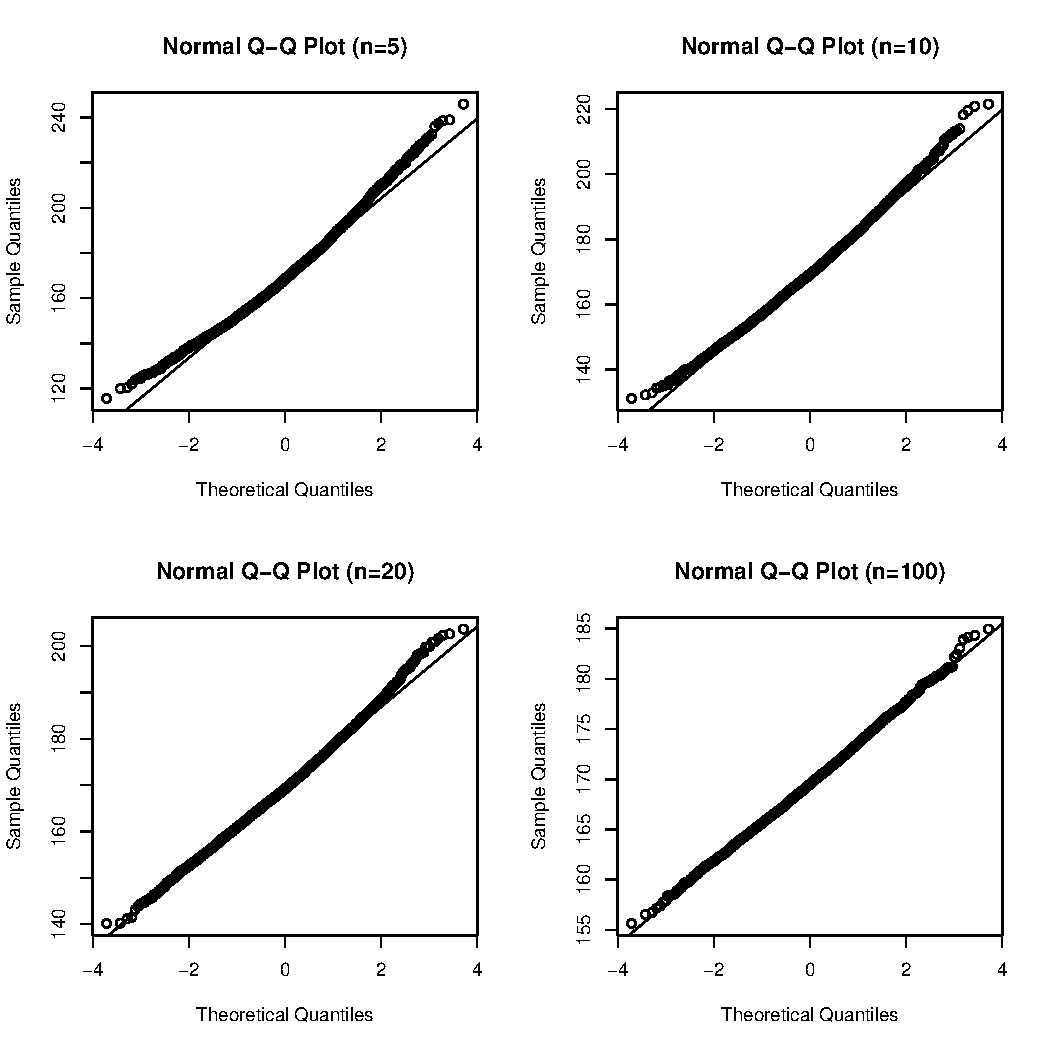
\includegraphics[width=\maxwidth]{figure/unnamed-chunk-8-1} 
\end{knitrout}


\begin{knitrout}
\definecolor{shadecolor}{rgb}{0.969, 0.969, 0.969}\color{fgcolor}\begin{kframe}
\begin{alltt}
\hlkwd{mean}\hlstd{(cdc}\hlopt{$}\hlstd{weight)} \hlcom{# population mean}
\end{alltt}
\begin{verbatim}
## [1] 169.683
\end{verbatim}
\begin{alltt}
\hlcom{# means of each sampling distribution}
\hlkwd{mean}\hlstd{(xbars5)}
\end{alltt}
\begin{verbatim}
## [1] 169.6472
\end{verbatim}
\begin{alltt}
\hlkwd{mean}\hlstd{(xbars10)}
\end{alltt}
\begin{verbatim}
## [1] 169.8427
\end{verbatim}
\begin{alltt}
\hlkwd{mean}\hlstd{(xbars20)}
\end{alltt}
\begin{verbatim}
## [1] 169.6234
\end{verbatim}
\begin{alltt}
\hlkwd{mean}\hlstd{(xbars100)}
\end{alltt}
\begin{verbatim}
## [1] 169.5839
\end{verbatim}
\begin{alltt}
\hlcom{# standard deviations of each sampling distribution}
\hlkwd{sd}\hlstd{(xbars5)}
\end{alltt}
\begin{verbatim}
## [1] 18.00604
\end{verbatim}
\begin{alltt}
\hlkwd{sd}\hlstd{(cdc}\hlopt{$}\hlstd{weight)} \hlopt{/} \hlkwd{sqrt}\hlstd{(}\hlnum{5}\hlstd{)}
\end{alltt}
\begin{verbatim}
## [1] 17.92475
\end{verbatim}
\begin{alltt}
\hlkwd{sd}\hlstd{(xbars10)}
\end{alltt}
\begin{verbatim}
## [1] 12.71319
\end{verbatim}
\begin{alltt}
\hlkwd{sd}\hlstd{(cdc}\hlopt{$}\hlstd{weight)} \hlopt{/} \hlkwd{sqrt}\hlstd{(}\hlnum{10}\hlstd{)}
\end{alltt}
\begin{verbatim}
## [1] 12.67472
\end{verbatim}
\begin{alltt}
\hlkwd{sd}\hlstd{(xbars20)}
\end{alltt}
\begin{verbatim}
## [1] 8.934549
\end{verbatim}
\begin{alltt}
\hlkwd{sd}\hlstd{(cdc}\hlopt{$}\hlstd{weight)} \hlopt{/} \hlkwd{sqrt}\hlstd{(}\hlnum{20}\hlstd{)}
\end{alltt}
\begin{verbatim}
## [1] 8.962377
\end{verbatim}
\begin{alltt}
\hlkwd{sd}\hlstd{(xbars100)}
\end{alltt}
\begin{verbatim}
## [1] 3.973856
\end{verbatim}
\begin{alltt}
\hlkwd{sd}\hlstd{(cdc}\hlopt{$}\hlstd{weight)} \hlopt{/} \hlkwd{sqrt}\hlstd{(}\hlnum{100}\hlstd{)}
\end{alltt}
\begin{verbatim}
## [1] 4.008097
\end{verbatim}
\end{kframe}
\end{knitrout}

\clearpage

\textbf{Remark}: We can also generate a sampling distribution for other statistics such as the median.

\begin{knitrout}
\definecolor{shadecolor}{rgb}{0.969, 0.969, 0.969}\color{fgcolor}\begin{kframe}
\begin{alltt}
\hlkwd{set.seed}\hlstd{(}\hlnum{999}\hlstd{)}
\hlstd{meds} \hlkwb{<-} \hlkwd{rep}\hlstd{(}\hlnum{0}\hlstd{,} \hlnum{5000}\hlstd{)}
\hlkwa{for}\hlstd{(i} \hlkwa{in} \hlnum{1}\hlopt{:}\hlnum{5000}\hlstd{) \{}
  \hlstd{samp} \hlkwb{<-} \hlkwd{sample}\hlstd{(cdc}\hlopt{$}\hlstd{weight,} \hlnum{30}\hlstd{)}
  \hlstd{meds[i]} \hlkwb{<-} \hlkwd{median}\hlstd{(samp)}
\hlstd{\}}

\hlkwd{par}\hlstd{(}\hlkwc{mfrow}\hlstd{=}\hlkwd{c}\hlstd{(}\hlnum{1}\hlstd{,}\hlnum{2}\hlstd{),} \hlkwc{cex}\hlstd{=}\hlnum{0.6}\hlstd{)}
\hlkwd{hist}\hlstd{(meds,} \hlkwc{main}\hlstd{=}\hlstr{"Histogram of Sample Medians (n=30)"}\hlstd{)}
\hlkwd{qqnorm}\hlstd{(meds)}
\hlkwd{qqline}\hlstd{(meds)}
\end{alltt}
\end{kframe}
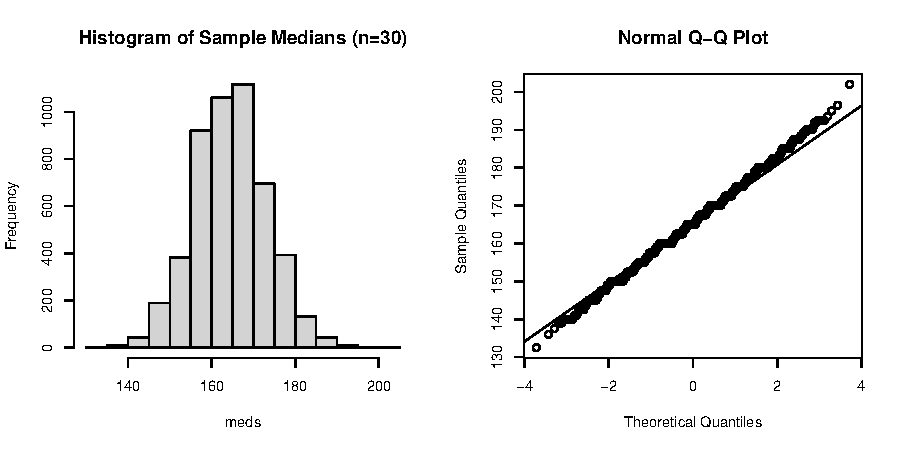
\includegraphics[width=\maxwidth]{figure/unnamed-chunk-10-1} 
\end{knitrout}




\end{document}
